\section{The lattice}\label{sec:lbm:lattice}
The discrete spatial coordinates together with the discrete velocity
coordinates forms a lattice. Spatial coordinates are neighborwise
connect through the discrete velocities. The discretisation in the LBM
must be performed in such a way that the lattice may be produced from
translating a single unit cell. This gives that the spatial resolution
is constant for the whole domain. In other approaches, e.g. finite
element methods the mesh may locally be refined at interesting regions
of the domain which is a strength to the LBM.  

There exist a convention for naming different lattices. A lattice of
dimension $d$ and with $q$ distinct velocities is denoted by
D$d$Q$q$. For example a lattice with 9 velocities in dimension 2 is
denoted D2Q9. An example of two different lattices is presented in
fig, \ref{fig:lbm:lattices}. The D2Q9 lattice is also the one that
will be used in this work, the velocities $\ci$ is given by

\begin{equation}\label{eq:lbm:d2q9_c}
\{\ci\} = \left\{
\begin{bmatrix}0\\0\end{bmatrix}, 
\begin{bmatrix}1\\0\end{bmatrix}, 
\begin{bmatrix}0\\1\end{bmatrix}, 
\begin{bmatrix}-1\\0\end{bmatrix}, 
\begin{bmatrix}0\\-1\end{bmatrix}, 
\begin{bmatrix}1\\1\end{bmatrix}, 
\begin{bmatrix}-1\\1\end{bmatrix}, 
\begin{bmatrix}-1\\-1\end{bmatrix}, 
\begin{bmatrix}1\\-1\end{bmatrix}
\right\} 
\end{equation}

\begin{figure}
  \centering
  \subfloat[D2Q7
    ]{\label{fig:lbm:q7}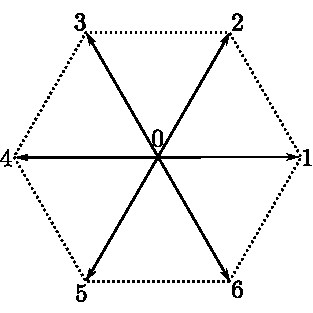
\includegraphics[width=0.4\textwidth]{fig/lattice_d2q7.pdf}}      
  \hspace{15pt} \subfloat[D2Q9
  ]{\label{fig:lbm:q9}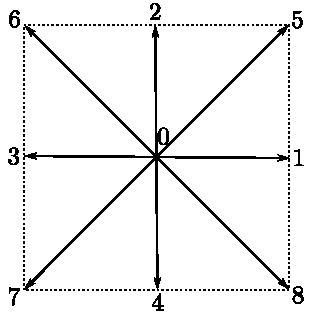
\includegraphics[width=0.38\textwidth]{fig/lattice_d2q9.pdf}
  }
  \caption{Two different unit cells for lattices used in the LBM in two
    dimensions. In (a) the D2Q7 seven speed lattice is shown and in
    (b) the nine speed D2Q9 lattice. The numbering at the edges is the
    usual naming convention for the different velocities.}
  \label{fig:lbm:lattices}
\end{figure}
 
To be able to retrieve the desired equations in the macroscopic limit
of the LBE, the lattice used must possess a certain degree of
isotropy. Thus the choice of lattice is not arbitrary. For instance,
for obtaining the Navier-Stokes equations, the lattice must at least
posses the following properties:

\begin{equation}\label{eq:lbm:i1}
\sum_i w_i = 1
\end{equation} 

\begin{equation}\label{eq:lbm:i2}
\sum_i w_ic_{i\alpha} = 0
\end{equation}

\begin{equation}\label{eq:lbm:i3}
\sum_i w_ic_{i\alpha}c_{i\beta} = c_s^2\delta_{\alpha \beta}
\end{equation}

\begin{equation}\label{eq:lbm:i4}
\sum_i w_ic_{i\alpha}c_{i\beta}c_{i\gamma} = 0
\end{equation}
where the sums are over the discrete velocities $\ci$, $w_i$ are
lattice specific weights $c_s$ is the sound of speed for the lattice
and $\delta_k$ is Kroenecker's delta. 

The weights are introduced to compensate for the fact that different
velocity vectors $\ci$ is of different length. See for example the
D2Q9 lattice in fig. \ref{fig:lbm:q9} where three lengths are
present. In this case, three different weights will be needed. From
the relations in eqs. \eqref{eq:lbm:i1}\eqref{eq:lbm:i4} follow that
these weights are: 
\begin{equation}\label{eq:lbm:weights}
w_i = 
\left\{
  \begin{array}{l l}
    4/9 & \quad \text{if $i = 0$}\\ 
    1/9 & \quad \text{if $i = 1, 2, 3, 4$}\\    
    1/36 & \quad \text{if $i = 5, 6, 7, 8$}\\
  \end{array} \right.
\end{equation}
The quantity $c_s$ which often is referred to as the speed of sound is
determined to 

\begin{equation}
c_s = c/3
\end{equation} 
where $c = |\mathbf{c}_{1,2,3,4}| = \delta_x/\delta_t$.
